\documentclass{article}
\usepackage{tikz,times}
\usepackage[paperwidth=25cm,paperheight=22cm,left=1cm,top=1cm]{geometry}

\usetikzlibrary{mindmap,backgrounds}

\pagestyle{empty}

\begin{document}
\centering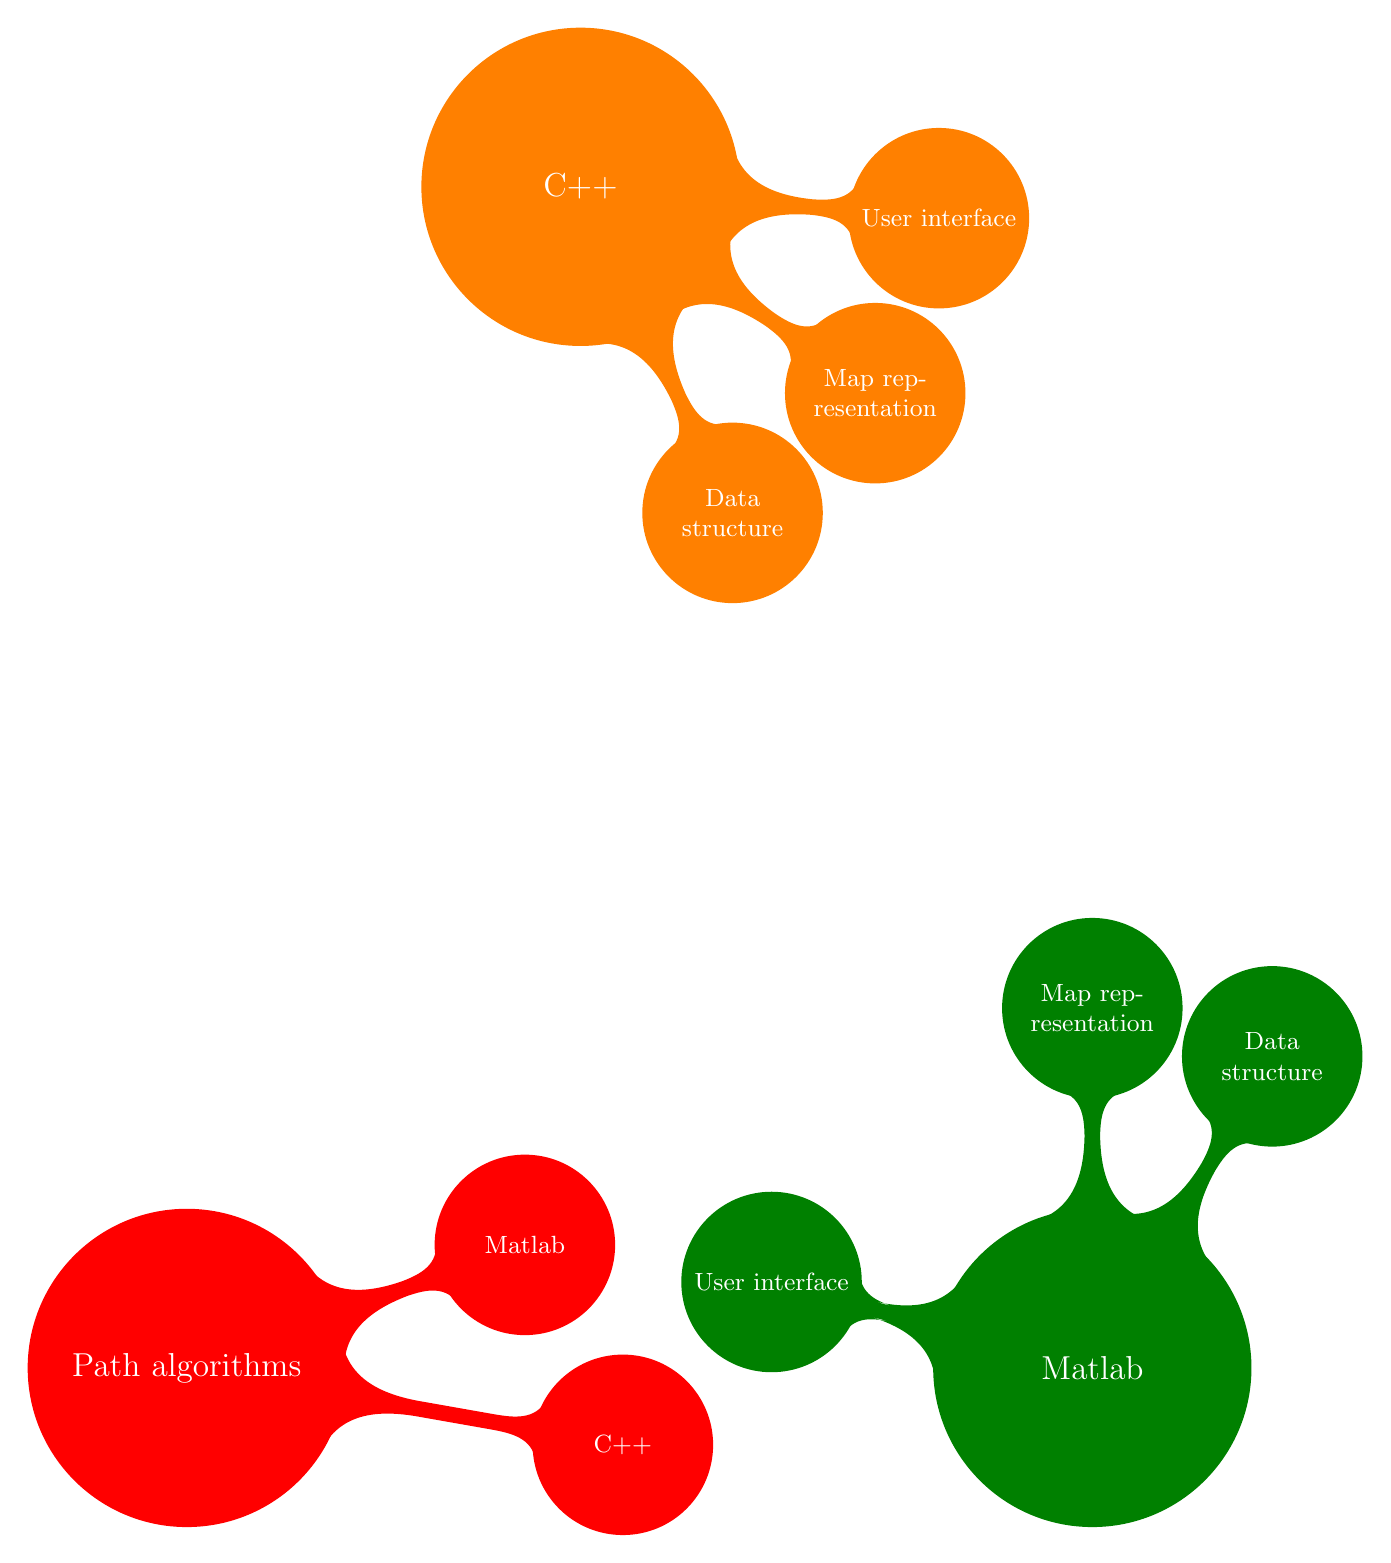
\begin{tikzpicture}[mindmap,
  level 1 concept/.append style={level distance=130,sibling angle=30},
  extra concept/.append style={color=blue!50,text=black}]

  % C++

  \begin{scope}[mindmap, concept color=orange, text=white]
    \node [concept] {C++}[clockwise from=-5] 
      child {node [concept] (log) {User interface}}
      child {node [concept] (alg) {Map representation}}
      child {node [concept] (cod) {Data structure}};
  \end{scope}

  % PATH algorithm

  \begin{scope}[mindmap, concept color=red,text=white]
    \node [concept] at (-5,-15) {Path algorithms}
      child [grow=-10, level distance=160]
        {node [concept] (qin) {C++}}
      child [grow=20] 
        {node [concept] (csm) {Matlab}};
  \end{scope}

  % Matlab

  \begin{scope}[mindmap, concept color=green!50!black,text=white]
    \node [concept] at (6.5,-15) {Matlab} 
      child [grow=165, level distance=120] 
        {node [concept] (med) {User interface}}
      child [grow=90] 
        {node [concept] (gen) {Map representation}}
      child [grow=60] 
        {node [concept] (aa) {Data structure}};
        
  \end{scope}

 

  % Connections of researchers to applied subfields

%  \begin{pgfonlayer}{background}
%    \draw [circle connection bar]
%      (kab) edge (cod)
%      (kch) edge (alg) edge (gen)
%      (lhc) edge (med)
%      (ksh) edge (dec)
%      (ndr) edge (mat)
%      (otr) edge (opt) edge (csm) edge (img)
%      (raf) edge (alg) edge (gen)
%      (rbk) edge (res) edge (mat)
%      (sht) edge (log) edge (dec)
%      (ver) edge (qin) edge (cod);
%  \end{pgfonlayer}
\end{tikzpicture}

\end{document}